\section{Experimental evaluation}
\label{section:experiments}



In Figure~\ref{fig:arch} we show the general view of the architecture and in 
Figure~\ref{fig:prototype} we show working prototype.

\begin{figure}[!h]
        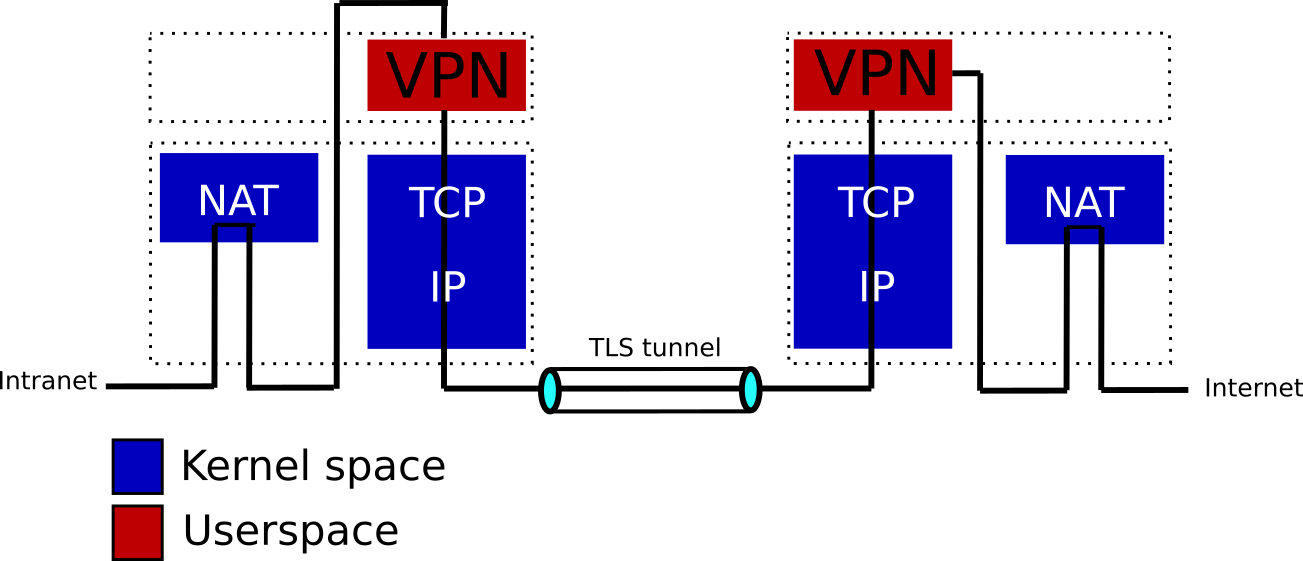
\includegraphics[width=0.5\textwidth]{graphics/architecture.png}
        \caption{Architecture of the prototype}
        \label{fig:arch}
\end{figure}

\begin{figure}[!h]
        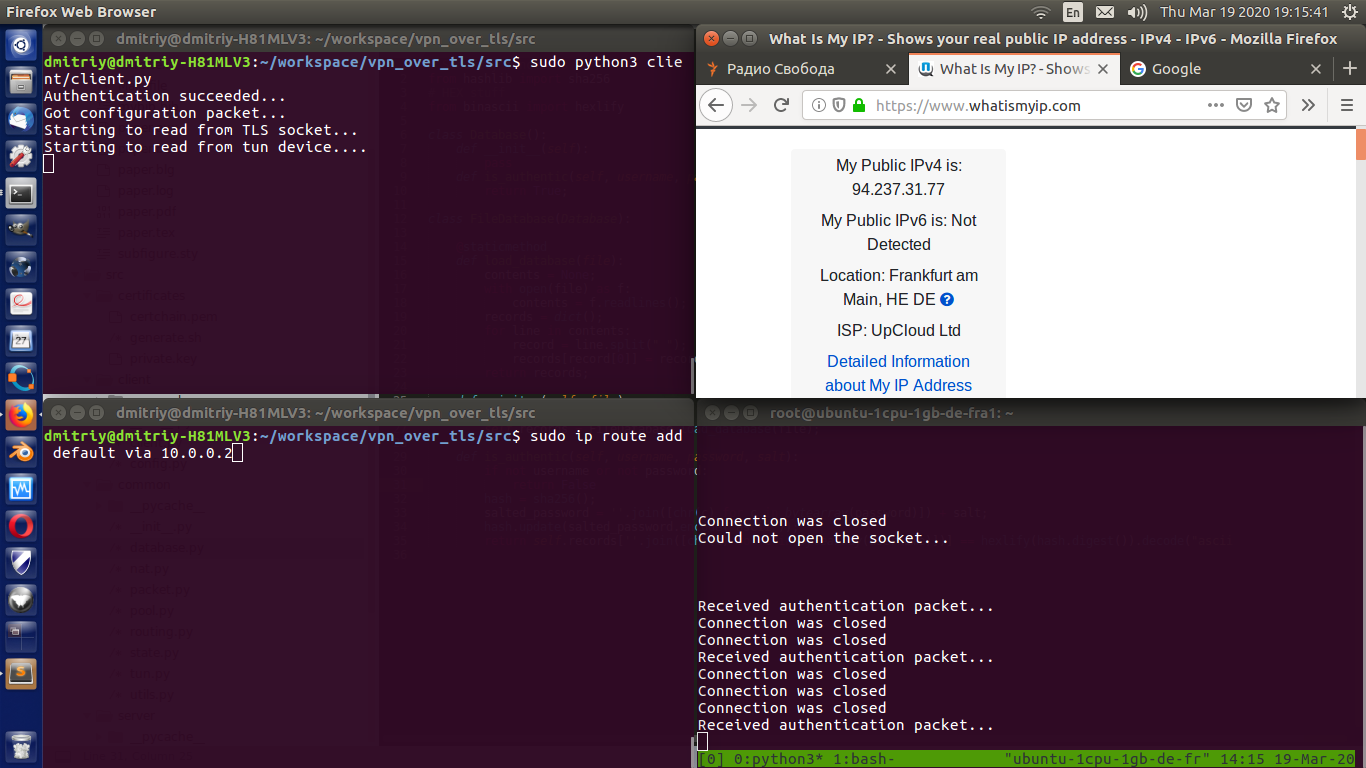
\includegraphics[width=0.5\textwidth]{graphics/vpn_over_tls_prototype.png}
        \caption{Working prototype}
        \label{fig:prototype}
\end{figure}

We have made several experiments over the course of our work. The very first experiment was 
related to sending ping messages towards the VPN TLS server and observing the differences in
round trip times (basically, we have compared the round trip times between the setting in 
which tunnel was present and the setting in which the tunnel did not exist). Next, we have
sat down to measure the throughput between the local and remote machine. Basically, we have 
performed $50$ measurements for a setting, in which the traffic was going inside the tunnel
and the same number of measurements for the setting, in which the traffic was going 
normally (meaning, unencrypted and not encapsulated in TLS packets).

In Figure~\ref{fig:rtt} we show the distribution of round-trip times
(RTT). Obviously, the distributions are similar, and RTT for
plain ICMP packets just slightly smaller.

\begin{figure}[!h]
        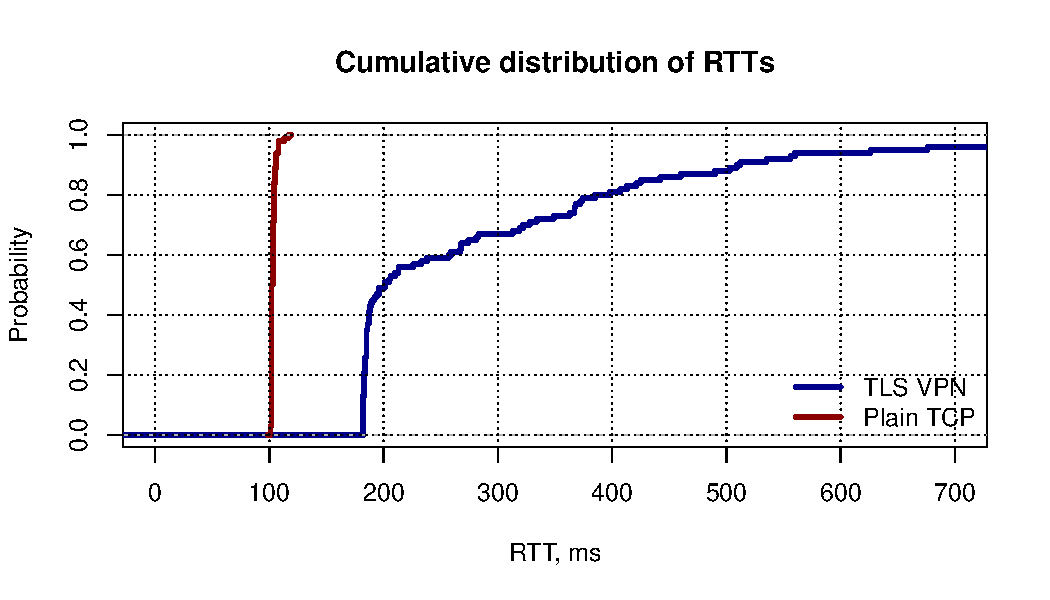
\includegraphics[width=0.5\textwidth]{graphics/rtt.pdf}
        \caption{Distribution of RTTs}
        \label{fig:rtt}
\end{figure}

In Figure~\ref{fig:iperf_distr} we show the distribution of the obtained throughput for both
TLS protected tunnel and regular TCP connections. Mean value for the VPN connection was 
$6.4$ Mb/s, and mean throughput for plain TCP connection was $12.06$ Mb/s. Obviously, 
TCP inside TCP and userspace implementation of VPN client and server, decreases the 
throughput considerably.

\begin{figure}[!h]
        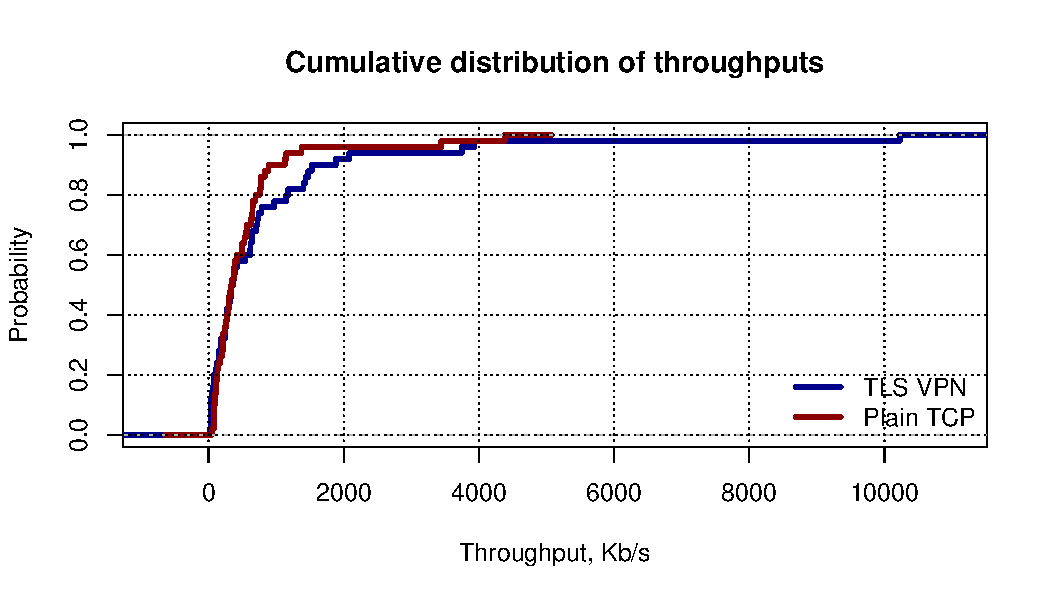
\includegraphics[width=0.5\textwidth]{graphics/throughput.pdf}
        \caption{Distribution of throughputs}
        \label{fig:iperf_distr}
\end{figure}

Finally, we have made a successful experiment in which the tunnel was used for a long period of time
without interruption (the tunnel was used for about 6 hours).
